\section{The mixing law}
\label{app:law}
\subsection{Precise statement}
On $n$ traceless coordinates let the step be $r_t=(1-p)O(u_t)r_{t-1}+pb$, where independent, identically
distributed inputs select orthogonal maps $O(u)$ and $b$ represents the reset state. Assume that the mean map
$A=\mathbb EO$ has spectral radius below one, that the only symmetric matrices fixed by
$X\mapsto\mathbb E[OXO^{\mathsf T}]$ are multiples of the identity, and that the input writes a signal,
$\mathbb E\|(O-A)(1-A)^{-1}b\|^2>0$. For a fixed linear readout of positive rank, draw the order $D_p$ with
probability equal to its share of the ideal memory. Then $pD_p\to\mathrm{Exp}(2/s)$ in distribution with
$s=1-\|A\|_F^2/n$, and $\mathbb ED_p=s/(2p)+O(1)$.

\emph{Idea.} One input writes a variance of order $p^2$. A covariance shape that survives for $1/(2p)$ steps
collects it to order $p$. We identify that shape and then count, with the recursion of
Eq.~\eqref{eq:recursion}, how many inputs it contains.

\subsection{Generating function}
\label{app:gen}
The order transfer $\mathcal F=(1-\mathcal B)^{-1}\mathcal K$ is a positive map on covariance matrices, and
$(1-\mathcal F)^{-1}=(1-\mathcal T)^{-1}(1-\mathcal B)=1+(1-\mathcal T)^{-1}\mathcal K$ is positive, so its spectral
radius is below one. Summing Eq.~\eqref{eq:recursion},
\begin{equation}
\begin{aligned}
  \sum_{k\ge1}z^kG_k&=z(1-z\mathcal F)^{-1}G_1,\\
  \sum_{k\ge1}kG_k&=(1-\mathcal F)^{-1}\Sigma ,
\end{aligned}
  \label{eq:generating}
\end{equation}
and $\mathcal F^K\Sigma$ is the covariance above order $K$.

\subsection{The surviving covariance}
\label{app:cov}
Let $r=1-p$, $A=\mathbb EO$, $\mathcal B_0X=AXA^{\mathsf T}$ and $\mathcal T_0X=\mathbb E[OXO^{\mathsf T}]$. Every step
contracts differences by $r$, so there is a unique stationary state. Its mean is $m_p=p(1-rA)^{-1}b=p\mu+O(p^2)$
with $\mu=(1-A)^{-1}b$, and the innovation $\xi_p=r(O-A)m_p$ has covariance $V_p=p^2V_0+O(p^3)$ with
$v=\Tr V_0=\|\mu\|^2-\|A\mu\|^2>0$ by the writing assumption. On symmetric matrices $\mathcal T_0$ preserves the trace
and the identity and contracts the Frobenius norm; by assumption the identity is its only fixed point, and power
boundedness excludes a Jordan block. Its spectral projector is $X\mapsto1\,\Tr X/n$, and all other directions have
a bounded resolvent near one. Hence
\begin{equation}
  \Sigma_p=(1-r^2\mathcal T_0)^{-1}V_p=\frac{pv}{2n}\,1+O(p^2).
  \label{eq:slowcov}
\end{equation}
The mean map is mixing, so $(1-r^2\mathcal B_0)^{-1}$ stays bounded and every fixed order has $G_k=O(p^2)$. Since
$\Sigma_y^+=O(p^{-1})$ on its support, any fixed set of orders carries a share $O(p)$, while the shares add up to the
rank $q$ of the readout.

\subsection{The number of inputs}
\label{app:inputs}
At $p=0$ the transfer $\mathcal F_0=(1-\mathcal B_0)^{-1}(\mathcal T_0-\mathcal B_0)$ fixes the identity; it is
positive and power bounded, and its unit eigenvalue is simple. Its left eigenfunctional is
\begin{equation}
  \ell(X)=\Tr[(1-A^{\mathsf T}A)X],\quad \ell(1)=ns>0,
\end{equation}
because $\ell=\Tr\circ(1-\mathcal B_0)$ and $\Tr\circ\mathcal T_0=\Tr$. Differentiating
$(1-r^2\mathcal B_0)\mathcal F_p=r^2(\mathcal T_0-\mathcal B_0)$ at $p=0$ gives $(1-\mathcal B_0)\mathcal F_0'1=-2\cdot1$,
so the leading eigenvalue is $1-\beta p+O(p^2)$ with $\beta=2n/\ell(1)=2/s$. Insert $z=e^{-\lambda p}$ into
Eq.~\eqref{eq:generating}: for fixed $\lambda\ge0$ only this eigenvalue gives a divergent resolvent term, and with
$\ell(G_1)=p^2v+O(p^3)$,
\begin{equation}
  \sum_{k\ge1}e^{-\lambda pk}G_k=\frac{pv}{\ell(1)(\lambda+\beta)}\,1+O(p^2).
\end{equation}
Divided by Eq.~\eqref{eq:slowcov} this is the Laplace transform $\beta/(\lambda+\beta)$ of the exponential law.
The second identity in Eq.~\eqref{eq:generating} gives the order-weighted covariance $\Sigma_p/(\beta p)+O(p)$, hence
$\mathbb ED_p=1/(\beta p)+O(1)=s\,t_{\mathrm{mem}}+O(1)$.

\subsection{The mixing fraction}
For a unit vector $x$ drawn uniformly, $\mathbb E\|(O-A)x\|^2=\Tr\mathcal K_0(1)/n=s$: one input moves a fraction $s$ of
a stored signal away from the average turn, and this fraction is passed to the next order. For
$O=e^{u\theta G}$ with $u=\pm1$ and skew-symmetric $G$ with eigenvalues $i\lambda_j$, the mean map is $\cosh\theta G$
and $s=n^{-1}\sum_j\sin^2\theta\lambda_j$, which grows as $\theta^2$.

\subsection{Two sectors, two laws}
The assumption of a single fixed covariance matters. Let a classical flag select one of two qubit rotations about
$Z$, by $\pm\pi/6$ or $\pm\pi/3$, and let the reset state be block diagonal. Each sector obeys the law separately,
and a single $Y$ readout sees the mixture $\Pr(pD_p>x)\to\frac12e^{-8x}+\frac12e^{-8x/3}$.

\subsection{Physical channels}
\label{app:physical}
A physical channel does not reset to a prescribed state, but the argument above only needs a single slow
covariance direction. We state the general version that Appendix~\ref{app:spins} uses and prove it along the same
four steps.

\emph{Setting.} Work on invariant reachable coordinates and translate a common limiting fixed point to zero; for the
spin reservoir of Appendix~\ref{app:spins} these are the dark coordinates, which the bright part follows at order
$\epsilon$ [Eq.~\eqref{eq:slowstep}]. The step
is $r_t=A_{u_t}(\epsilon)r_{t-1}+b_{u_t}(\epsilon)$ with a small leakage $\epsilon$, and we write $\bar A_\epsilon=\mathbb E A_u(\epsilon)$,
$\mathcal B_\epsilon X=\bar A_\epsilon X\bar A_\epsilon^{\mathsf T}$, $\mathcal T_\epsilon X=\mathbb E[A_uXA_u^{\mathsf T}]$ and
$\mathcal K_\epsilon=\mathcal T_\epsilon-\mathcal B_\epsilon$. Assume:
(i) $A_u(\epsilon)=A_{u,0}+\epsilon A_{u,1}+O(\epsilon^2)$ and $b_u(\epsilon)=\epsilon b_{u,1}+O(\epsilon^2)$ in mean square;
(ii) the mean step is mixing at $\epsilon=0$, that is, $\bar A_0$ has spectral radius below one;
(iii) the channel is mean-square stable for small $\epsilon>0$;
(iv) $\mathcal T_\epsilon$ has a simple eigenvalue $1-\kappa\epsilon+O(\epsilon^2)$ with $\kappa>0$, all its other eigenvalues stay
a fixed distance away from one, and at $\epsilon=0$ the eigenvalue has right eigenmatrix $R\succeq0$ and a left
eigenfunctional $\ell$ of $\mathcal T_0$ that is nonnegative on positive matrices, with $\ell(R)=1$;
(v) the input writes along it, $\ell(V_*)>0$, where $V_*$ is defined in step 1.

\emph{Step 1: the innovation.} The stationary mean solves $m=\bar A_\epsilon m+\mathbb Eb_u(\epsilon)$. By (ii) it is
$m_\epsilon=\epsilon m_1+O(\epsilon^2)$ with $m_1=(1-\bar A_0)^{-1}\mathbb Eb_{u,1}$. The innovation is therefore
$\xi_u=\epsilon z_u+O(\epsilon^2)$ with $z_u=A_{u,0}m_1+b_{u,1}-m_1$, and its covariance is $V_\epsilon=\epsilon^2V_*+O(\epsilon^3)$ with
$V_*=\mathbb E[z_uz_u^{\mathsf T}]$; this is the order-$p^2$ writing of Appendix~\ref{app:cov}.

\emph{Step 2: the surviving covariance.} Let $\mathcal P_\epsilon$ be the spectral projector of the simple eigenvalue in (iv);
it depends smoothly on $\epsilon$ and $\mathcal P_0X=R\,\ell(X)$. On the complement $(1-\mathcal T_\epsilon)^{-1}$ stays bounded,
while on the slow direction it divides by $\kappa\epsilon+O(\epsilon^2)$. Since $\mathcal P_\epsilon V_\epsilon=\epsilon^2\ell(V_*)R+O(\epsilon^3)$,
\begin{equation}
\begin{aligned}
  \Sigma_\epsilon&=(1-\mathcal T_\epsilon)^{-1}V_\epsilon=\epsilon\,C_*+O(\epsilon^2),\\
  C_*&=\frac{\ell(V_*)}{\kappa}\,R .
\end{aligned}
\end{equation}

\emph{Step 3: every fixed order is small.} By (ii) the spectral radius of $\mathcal B_\epsilon$ stays below one, so
$(1-\mathcal B_\epsilon)^{-1}$ is bounded. Equation~\eqref{eq:recursion} then gives $G_1=O(\epsilon^2)$ and, since $\mathcal K_\epsilon$ is
bounded, $G_k=O(\epsilon^2)$ for every fixed $k$. Its share of the observed variance of a readout $M$ tends to zero
whenever $\Tr(MC_*M^{\mathsf T})>0$. For the ideal memory of a readout with several features we also need $MC_*M^{\mathsf T}$
to have full rank on the measured support, so that $(M\Sigma_\epsilon M^{\mathsf T})^+=O(\epsilon^{-1})$; for a single observable
this holds trivially.

\emph{Step 4: the number of inputs.} At $\epsilon=0$ the order transfer $\mathcal F_0=(1-\mathcal B_0)^{-1}\mathcal K_0$ has the same
fixed points as $\mathcal T_0$, because $\mathcal F_0X=X$ is equivalent to $(1-\mathcal B_0)X=\mathcal T_0X-\mathcal B_0X$. Its left fixed
functional is $\ell_F=\ell\circ(1-\mathcal B_0)$, since $\ell_F(\mathcal F_0X)=\ell(\mathcal K_0X)=\ell(X)-\ell(\mathcal B_0X)$. Define
\begin{equation}
  s=\ell_F(R)=\ell(\mathcal K_0R).
\end{equation}
Because $\mathcal K_0X=\mathbb E[(A_{u,0}-\bar A_0)X(A_{u,0}-\bar A_0)^{\mathsf T}]$, the matrix $\mathcal K_0R$ is positive and
$s=1-\ell(\mathcal B_0R)$ lies between 0 and 1; for the same reason $\ell(\mathcal B_0Y)\le\ell(\mathcal T_0Y)=\ell(Y)$ for every
$Y\succeq0$. If $s$ vanished, then $0\le\ell(\mathcal B_0^j\mathcal K_0R)\le s=0$ for every $j$, and the Neumann series
$\mathcal F_0=\sum_{j\ge0}\mathcal B_0^j\mathcal K_0$ would give $\ell(\mathcal F_0R)=0$, which contradicts $\mathcal F_0R=R$ and
$\ell(R)=1$. So $s>0$. The fixed space of $\mathcal F_0$ is spanned by $R$, and because $\ell_F(R)=s\neq0$ the eigenvalue one
has no Jordan chain, so it is simple. Differentiating $(1-\mathcal B_\epsilon)\mathcal F_\epsilon=\mathcal T_\epsilon-\mathcal B_\epsilon$ at $\epsilon=0$ and applying it to $R$
gives $(1-\mathcal B_0)\mathcal F_0'R=\mathcal T_0'R$, hence $\ell_F(\mathcal F_0'R)=\ell(\mathcal T_0'R)=-\kappa$. First-order
perturbation of the simple eigenvalue then gives the order eigenvalue
\begin{equation}
  \mu_\epsilon=1-\beta\epsilon+O(\epsilon^2),\qquad \beta=\frac{\kappa}{s}.
\end{equation}
Insert $z=e^{-\lambda\epsilon}$ into Eq.~\eqref{eq:generating}. The other eigenvalues of $\mathcal F_0$ have modulus at most
one, because by (iii) and the positivity argument of Appendix~\ref{app:gen} the spectral radius of $\mathcal F_\epsilon$ is
below one for $\epsilon>0$, and by the simplicity shown above they differ from one, so only $\mu_\epsilon$ gives a divergent
resolvent term. Since $G_1=(1-\mathcal B_\epsilon)^{-1}V_\epsilon$ and $\ell_F$ is taken at $\epsilon=0$,
$\ell_F(G_1)=\ell(V_\epsilon)+O(\epsilon^3)=\epsilon^2\ell(V_*)+O(\epsilon^3)$, and
\begin{equation}
\begin{aligned}
  \sum_{k\ge1}e^{-\lambda\epsilon k}G_k&=\frac{\epsilon\,\ell(V_*)}{s(\lambda+\beta)}\,R+O(\epsilon^2)\\
  &=\epsilon\,C_*\,\frac{\beta}{\lambda+\beta}+O(\epsilon^2).
\end{aligned}
\end{equation}
Divided by $\Sigma_\epsilon$ from step 2 this is the Laplace transform of $\mathrm{Exp}(\beta)$, for the share of observed
variance and, under the rank condition of step 3, for the ideal memory. The second identity in
Eq.~\eqref{eq:generating} gives $\mathbb ED_\epsilon=1/(\beta\epsilon)+O(1)=s/(\kappa\epsilon)+O(1)$: $s$ is the mixing
fraction of the channel and $1/(\kappa\epsilon)$ its memory time. For the reset model, $\mathcal T_p=(1-p)^2\mathcal T_0$ gives
$\kappa=2$, $R=1$ and $\ell=\Tr/n$, so $s=1-\|A\|_F^2/n$ and $\beta=2/s$ as in Appendix~\ref{app:inputs}.

\subsection{Numerical check}
Figure~\ref{fig:law} compares the law with exact moments. For each dimension $d=2,3,4$ we draw two families of three
Haar unitaries applied with probabilities $(0.2,0.3,0.5)$, each with two reset states (a basis state and a random pure
state) and two readouts (all coordinates or one random direction). Up to $K=\lceil6/(\beta p)\rceil$ we evaluate the
remaining share $\Tr[\Sigma_y^+M\mathcal F^K(\Sigma)M^{\mathsf T}]/q$. Over these 24 reservoirs and readouts the rates lie
between 2.89 and 4.00, and the largest deviation from $e^{-\beta pK}$ falls from 0.082 at $p=0.03$ to 0.0034 at
$p=0.001$; Fig.~\ref{fig:law} shows one of them.

\begin{figure}[t]
\centering
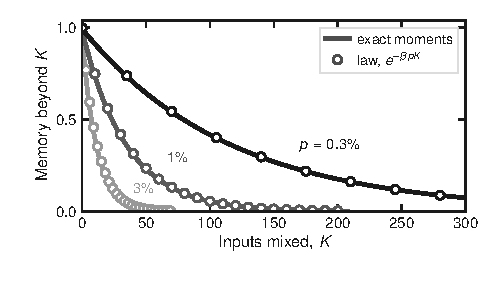
\includegraphics[width=\columnwidth]{figures/fig5_law.pdf}
\caption{\textbf{The mixing law.} Share of the ideal memory carried by products of more than $K$ inputs, for one
qubit reservoir with a reset to a basis state and a scalar readout, at reset probabilities $p=3\%$, 1\% and 0.3\%
(light to dark). Lines: exact moments; circles: the law $e^{-\beta pK}$ with $\beta=2/s=2.89$.}
\label{fig:law}
\end{figure}

\section{One qubit in closed form}
\label{app:qubit}
During one unit of time the qubit evolves under $u\theta Z/2$ and the jump $\sqrt\epsilon\,|{+x}\rangle\langle{-x}|$,
with signs $u=\pm1$, and is read along $Y$. In the Bloch plane, $\dot x=-\epsilon(x-1)-u\theta y$ and
$\dot y=u\theta x-\epsilon y/2$. For $u=+1$ write the step as
\begin{equation}
  e^{B}=\begin{pmatrix}a&-b\\ b&d\end{pmatrix},\qquad B=\begin{pmatrix}-\epsilon&-\theta\\ \theta&-\epsilon/2\end{pmatrix},
\end{equation}
with offset $(f,g)=\int_0^1e^{tB}(\epsilon,0)\,dt$; the opposite sign reverses $b$ and $g$. The stationary mean is
$(m,0)$ with $m=f/(1-a)$, and each input writes $u\,(0,v)$ with $v=bm+g$, along the measured axis.

The mean step is diagonal, while adding an input interchanges the two axes, so $Y$ carries only odd orders. By
Eq.~\eqref{eq:recursion} the variance passes from $y$ to $x$ with factor $b^2/(1-a^2)$ and back with $b^2/(1-d^2)$.
With $\chi$ their product,
\begin{equation}
\begin{aligned}
  C_{2j+1}&=(1-\chi)\chi^j, &\qquad \mathbb ED&=\frac{1+\chi}{1-\chi},\\
  \mathrm{Var}\,Y&=\frac{v^2}{(1-d^2)(1-\chi)},
\end{aligned}
\end{equation}
and the share of single past inputs is $d^2(1-\chi)$.
At fixed $\theta$ with $\sin\theta\neq0$, $1-\chi=3\epsilon/\sin^2\theta+O(\epsilon^2)$, so
$\epsilon D\to\mathrm{Exp}\bigl(3/(2\sin^2\theta)\bigr)$ and the share of single inputs vanishes even for exact
expectation values. If instead $\theta^2/\epsilon\to\nu>0$, then $a=1-(1+\nu/2)\epsilon$, $d=1-(1+\nu)\epsilon/2$ to first
order, $b\sim\theta$, $f\sim\epsilon$ and
\begin{equation}
  \chi\to\frac{\nu^2}{(\nu+2)(\nu+1)},\quad \mathrm{Var}\,Y\to\frac{4\nu}{(\nu+2)(3\nu+2)} .
\end{equation}
The mean order stays finite, the share of single past inputs tends to $1-\chi$, and since the recall beyond delay
$\tau$ is the fraction $d^{2\tau}$, the range obeys $\epsilon\tau_{90}\to\ln10/(1+\nu)$. The variance peaks at
$\nu=2/\sqrt3$. For
$\theta^2\gg\epsilon$ it vanishes as $4\epsilon/(3\theta^2)$ and for $\theta^2\ll\epsilon$ as $\theta^2/\epsilon$, so among power
laws for the angle only $\theta\propto\sqrt\epsilon$ keeps a finite signal. Density-matrix propagation reproduces these
expressions to relative error below $10^{-12}$ at 25 parameter pairs.

\section{The three-spin reservoir at strong loss}
\label{app:spins}
\emph{Idea.} At strong loss one step of the full master equation is, up to corrections of order $\epsilon=1/\gamma$, a
rotation of the dark subspace. With a fixed amplitude the two signs rotate differently; a single slow covariance
builds up, and the physical-channel version of the mixing law applies. With a scaled amplitude both signs give nearly
the same
rotation; the signal is written on the scale of the leakage and accumulates in six slow directions, which we follow
explicitly. Both arguments end in finitely many strict inequalities, which we enclose in interval arithmetic.

\subsection{What is proven}
For the four Hamiltonians of Table~\ref{tab:spins} and every Hamiltonian whose three couplings lie within $1/32$ of
theirs: with $\eta=1$, the order of the $X_1$ memory divided by $\gamma$ becomes exponentially distributed with a rate
$\beta_{\mathrm{spin}}$, and the variance of $X_1$ falls as $1/\gamma$. For the same four Hamiltonians and couplings
within $1/512$: with $\eta=8/\sqrt\gamma$, the recall of single past inputs from $X_1$ tends to a positive constant, and
its range divided by $\gamma$ tends to a positive constant.

\begin{table}[t]
\caption{\label{tab:spins}Strong-loss limits for $X_1$ in the four three-spin reservoirs: rate of the order
distribution at $\eta=1$ (certified); share of single past inputs and range at $\eta=8/\sqrt\gamma$, evaluated at
$\gamma=2^{16}$.}
\centering\footnotesize
\begin{tabular}{lccc}
\toprule
 & $\beta_{\mathrm{spin}}$ & single-input share & range$/\gamma$\\\midrule
H1 & 78.6 & 0.81 & 0.50\\
H2 & 91.7 & 0.29 & 0.18\\
H3 & 61.4 & 0.08 & 0.24\\
H4 & 132.5 & 0.14 & 0.50\\
\bottomrule
\end{tabular}

\end{table}

\subsection{The slow part of a step}
Let $\mathcal D$ be the dissipator at unit loss. Its dark space is spanned by the vacuum and the
single-excitation states with coefficients $(0,1,-1)/\sqrt2$ and $(2,1,1)/\sqrt6$; the jump is injective on two and
three excitations, so the kernel of $\mathcal D$ consists of the nine operators on the dark qutrit and all other
eigenvalues have negative real part. With $R$ embedding a Hermitian dark basis, $R^\flat=R^{\mathsf T}(\mathcal D+RR^{\mathsf T})^{-1}$,
$\mathcal P=RR^\flat$ and $\mathcal S=(\mathcal D+\mathcal P)^{-1}-\mathcal P$, perturbing the zero block of
$\mathcal D+\epsilon\mathcal H_u$ gives
\begin{equation}
  e^{\Delta t(\mathcal D/\epsilon+\mathcal H_u)}=RE_uR^\flat+\epsilon Z_u+O(\epsilon^2),
  \label{eq:slowstep}
\end{equation}
with $E_u=e^{\Delta t\,R^\flat\mathcal H_uR}$,
where $Z_u$ contains the two boundary terms $-\mathcal S\mathcal H_uRE_uR^\flat$ and $-RE_uR^\flat\mathcal H_u\mathcal S$ and the
leak $-\Delta t\,R^\flat\mathcal H_u\mathcal S\mathcal H_uR$ inside the exponential.

\subsection{Fixed amplitude}
At $\eta=1$ the dark rotations $O_u$ of the two signs differ. Two finite tests show that their mean is mixing and that
the identity is the only fixed dark covariance: $\|\bar O^{4096}\|_F<0.013$, and $1-T_D+vv^{\mathsf T}$ is invertible,
where $T_DX=\mathbb E[O_uXO_u^{\mathsf T}]$ and $v=1/\sqrt8$. The first-order terms of Eq.~\eqref{eq:slowstep} give the
writing strength $w$, the decay rate $\kappa$ of the slow covariance and the mixing fraction
$s_0=1-\|\bar O\|_F^2/8$, all certified positive. The physical-channel version of the mixing law then gives
$\beta_{\mathrm{spin}}=\kappa/s_0$, and the variance of $X_1$ is $\tfrac43(w/\kappa)\epsilon+O(\epsilon^2)$ because $X_1$
has overlap $1/6$ with the slow covariance. Throughout the boxes of half-width $1/32$, a coupling change $r$ moves each
dark rotation by at most $3r$, and ball arithmetic keeps $w$, $\kappa$ and $s_0$ above 0.0001, 3.53 and 0.052.

\subsection{Scaled amplitude}
At $\eta=g\sqrt\epsilon$, $g=8$, both signs give the same leading rotation $E$. A block exponential of the static,
drive and leak generators gives the mean step $E+\epsilon E_1$ and the fluctuating part $u\sqrt\epsilon D_1$. The six
coherence phases of the static dark Hamiltonian are separated from one another and from one, so the unit-eigenvalue
space of $E$ contains only populations, on which $E_1$ generates a population dynamics with a unique stationary state
$m_*$. The inputs therefore write $\pm\sqrt\epsilon\,v$ with $v=D_1m_*$, which lies in the coherence planes. The fixed
covariances of the rotation form a six-dimensional space: three population covariances and one identity per coherence
plane. On it the first-order generators
\begin{equation}
\begin{aligned}
  K_BX&=\mathcal P_6(E_1'XO^{\mathsf T}+OXE_1'^{\mathsf T}),\\
  K_TX&=K_BX+\mathcal P_6(D_1'XD_1'^{\mathsf T})
\end{aligned}
\end{equation}
are certified stable, and the summed linear response and the full covariance converge to $W_*=-K_B^{-1}\mathcal P_6(vv^{\mathsf T})$
and $\Sigma_*=-K_T^{-1}\mathcal P_6(vv^{\mathsf T})$. The recall of single inputs from $X_1$ tends to
$a^{\mathsf T}W_*a/a^{\mathsf T}\Sigma_*a$, and after $t/\epsilon$ steps the remaining fraction is
$a^{\mathsf T}e^{tK_B}W_*a/a^{\mathsf T}W_*a$, which crosses $0.1$ once; this crossing is the range divided by $\gamma$.
Interval tests bracket it to $4\times10^{-6}$. The certificates show $a^{\mathsf T}W_*a>0$, and since
$\Sigma_*\succeq W_*$ the limiting share is positive; the archived certificates state this numerator bound through the
recall of a readout with 1000 shots, which has the same numerator. On the boxes of half-width $1/512$, Sturm counts
and Weyl's bound keep the six phases separated and $-(K+K^{\mathsf T})$ positive definite for both generators, so the
limits stay positive.

The single-input shares in Table~\ref{tab:spins} range from 0.08 to 0.81 because the limit compares two rates of the
same order in $\epsilon$: $K_B$, at which the mean step lets a stored signal decay, and the extra term of $K_T$, at
which the random signs of later inputs turn it into products. Their ratio depends on the couplings through the dark
energies and the matrix elements of $X_1$ between dark states, so the mean order in the limit runs from 1.4 for H1 to
5.9 for H3. The boxes are 16 times narrower than for the fixed amplitude because this argument follows the dark
energy eigenstates themselves: a coupling change $r$ moves each eigenprojector by up to $3r/(\delta-3r)$, where $\delta$ is the
smallest gap between dark energies, whereas the fixed-amplitude argument needs only the rotations, which move by at
most $3r$.

\subsection{Erasing coherence}
Returning bright population to the dark subspace after every step leaves the leading terms of the scaled step
unchanged, so it keeps the same limits. Dephasing in the dark energy basis removes the coherence planes into which
$v$ writes. Restricted to populations, the two signs then differ only at order $\epsilon^{3/2}$, because the
order-$\sqrt\epsilon$ response of a diagonal state is off-diagonal, while the populations still follow $1+\epsilon L$.
A new input therefore writes a vector of size $\epsilon^{3/2}$, the slow dynamics accumulate its square over
$1/\epsilon$ steps, and the stored signal is $O(\epsilon^2)$.

\subsection{Certificates}
The attached archive \texttt{spin\_certificates.zip} contains the generators, the exact couplings and the interval
programs. At 192-bit precision they reproduce the archived enclosures; at 256 bits they check every strict inequality
above. An independent implementation (see Author contributions) that builds the full finite-rate maps and
extrapolates to infinite loss agrees
with the certified rates to $2\times10^{-7}$ and with the limiting recalls to $4\times10^{-9}$.

\section{Results of the first version}
\label{app:v1}
Table~\ref{tab:v1} repeats the benchmark comparison of the first version~\cite{BaumannV1} at $\gamma=1$, where the
same jump families have the same total coupling. The shared channel had the largest memory and the smallest NARMA-10
error but scored below local loss on parity and on closed-loop Mackey--Glass forecasting, two tasks that need products
of past inputs; at this operating point it also led local loss in memory and NARMA-10 error from four to eight spins.
Figure~\ref{fig:v1} repeats its finite-sampling test: when the 45 features are estimated from a finite number of
preparations per step, the advantage of the shared channel over local loss becomes significant only above about
$2\times10^5$ preparations per step if all spins are read in three grouped settings, and only above about
$3\times10^6$ if every feature is measured separately.

\begin{table}[h]
\caption{\label{tab:v1}Benchmark scores of the first version~\cite{BaumannV1} at $\gamma=1$, $h=\Delta t=1/2$, five
spins and 45 features, for parity read at 15 times within each step: mean over 32, 32, 16 and 64 reservoirs, with the standard error in the last digits in
parentheses. Memory sums $C_\tau$ over delays 1 to 20 and parity sums a capacity over windows of one to seven inputs
(larger is better); NARMA-10 and Mackey--Glass forecasting (MG) over 150 closed-loop steps are normalized errors
(smaller is better). The rows are those of the six jump families studied here; bold marks the best of them.}
\centering\footnotesize\setlength{\tabcolsep}{4pt}
\begin{tabular}{lllll}
\toprule
family & memory & NARMA-10 & parity & MG\\\midrule
local & 8.63(7) & 0.315(8) & 4.82(4) & \textbf{0.037(3)}\\
shared & \textbf{12.21(10)} & \textbf{0.229(6)} & 3.78(3) & 0.097(9)\\
pairwise & 9.20(8) & 0.289(7) & 4.75(4) & 0.039(4)\\
gain/loss & 8.31(6) & 0.337(8) & 4.85(4) & 0.046(4)\\
exchange & 7.41(5) & 0.441(9) & \textbf{5.08(5)} & 0.052(4)\\
dephasing & 0 & 1.020(6) & 0 & 0.0599(4)\\
\bottomrule
\end{tabular}
\end{table}

\begin{figure}[h]
\centering
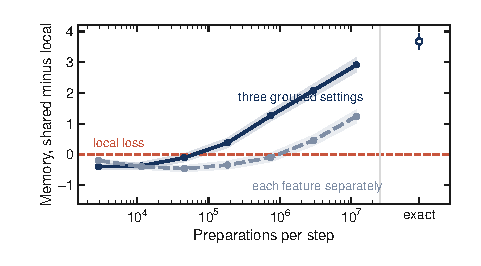
\includegraphics[width=\columnwidth]{figures/fig6_sampling.pdf}
\caption{\label{fig:v1}\textbf{Finite sampling in the first version.} Memory of one shared channel minus that of
local loss at $\gamma=1$ when every feature is estimated from a finite number of preparations per step, with all spins
read along $X$, $Y$ or $Z$ in three grouped settings (solid) or each feature measured separately (dashed). Lines and
bands show the mean and 95\% interval over 20 reservoirs; the open circle is exact. Data from
Ref.~\cite{BaumannV1}.}
\end{figure}

